\subsection{Aufgabestellung}

Das Projekt beschäftigt sich mit den Eigenschwingeungen einer fest eingespannten Saite. Sei dazu $u(t, x)$ die vertikale Auslenkung der Saite an der Position $x \in [0, 1]$ zur Zeit $t$. $u$ wird näherungsweise durch die sogenannte Wellengleichung

\begin{align} \label{Wellengleichung}
  \frac{\partial^2 u}{\partial x^2} (t, x) =
  \frac{1}{c^2}
  \frac{\partial^2 u}{\partial t^2} (t, x)
\end{align}

für alle $x \in (0, 1)$ und $t \in \R$ beschrieben, wobei $c$ die Ausbreitungsgeschwindigkeit der Welle ist. Wenn die Saite an beiden Enden fest eingespannt ist, so gelten die Randbedingungen

\begin{align*}
  u(t, 0) = u(t, 1) = 0
\end{align*}

für alle $t \in \R$. \\

Zur Berechnung der Eigenschwingungen suchen wir nach Lösungen $u$, die in der Zeit harmonisch schwingen. Solche erfüllen folgenden Ansatz

\begin{align*}
  u(x, t) = \mathfrak{R} (v(x) e^{-i \omega t})
\end{align*}

mit einer festen, aber unbekannten Kreisfrequenz $\omega > 0$ und einer Funktion $v$, welche nur noch vom Ort $x$ abhängt. Durch Einsetzen erhalten wir für $v$ die sogenannte Helmholz-Gleichung

\begin{align} \label{Helmholz-Gleichung}
  -v^\primeprime(x) = \kappa^2 v(x), \qquad
  x \in (0, 1),
\end{align}

mit der unbekannten Wellenzahl $\kappa := \frac{\omega}{c}$ und den Randbedingungen

\begin{align} \label{Randbedingungen}
  v(0) = v(1) = 0.
\end{align}

\subsection{Analytische Lösung}

\begin{align}
  v_\kappa(x) = C_1 \cos{(\kappa x)} + C_2 \sin{(\kappa x)}, \qquad
  x \in [0, 1],
  \label{Analytische_Lösung}
\end{align}

mit beliebigen Konstanten $C_1, C_2$ löst die Helmholz-Gleichung \eqref{Helmholz-Gleichung}. Das erkennt man durch stumpfes Einsetzen.

\begin{multline*}
  - v_\kappa^\primeprime(x)
  = - \frac{\partial^2}{\partial x^2}
    (C_1 \cos{(\kappa x)} + C_2 \sin{(\kappa x)})
  = - \frac{\partial}{\partial x}
    (- C_1 \kappa \sin{(\kappa x)} + C_2 \kappa \cos{(\kappa x)}) \\
  = - (- C_1 \kappa^2 \cos{(\kappa x)} - C_2 \kappa^2 \sin{(\kappa x)})
  = \kappa (C_1 \cos{(\kappa x)} + C_2 \sin{(\kappa x)})
  = \kappa^2 v_\kappa(x)
\end{multline*}

Wir fragen uns, für welche $\kappa > 0$, Konstanten $C_1$ und $C_2$ existieren, sodass $v_\kappa$ auch die Randbedingungen \eqref{Randbedingungen} erfüllt.

\begin{align*}
  0 \stackrel{!}{=}
  \begin{cases}
    v_\kappa(0)
    = C_1 \cos{0} + C_2 \sin{0}
    = C_1 \\
    v_\kappa(1)
    = C_1 \cos{\kappa} + C_2 \sin{\kappa}
    = C_2 \sin{\kappa}
  \end{cases}
\end{align*}

Nachdem $\cos{0} = 1$ und $\sin{0} = 0$, erhält man, aus der oberen Gleichung, $C_1 = 0$. Mit der unteren Gleichung folgt aber auch $C_2 \sin{\kappa} = 0$. Wenn nun auch $C_2 = 0$, dann erhielte man die triviale Lösung $v_\kappa = 0$. Für eine realistischere Modellierung, d.h. $v_\kappa \neq 0$, müsste $\sin{\kappa} = 0$, also $\kappa \in \pi \Z$. \\

Das sind die gesuchten $\kappa > 0$. Sei nun eines dieser $\kappa$ fest. Offensichtlich ist $C_1 = 0$ eindeutig, $C_2 \in \R$ jedoch beliebig.

\subsection{Numerische Approximation}

Häufig lassen sich solche Probleme nicht analytisch lösen, sodass auf numerische Verfahren zurückgegriffen wird, welche möglichst gute Näherungen an die exakten Lösungen berechnen sollen. Als einfachstes Mittel dienen sogenannte Differenzenverfahren. Sei dazu $x_j := jh$, $j = 0, \ldots, n$ eine Zerlegung des Intervalls $[0, 1]$ mit äquidistanter Schrittweite $h = 1/n$. Die zweite Ableitung in \eqref{Helmholz-Gleichung} wird approximiert durch den Differenzenquotienten

\begin{align} %\label{Differenzenquotient}
  v^\primeprime(x_j) \approx
  D_h v(x_j) :=
  \frac{1}{h^2} (v(x_{j-1}) - 2 v(x_j) + v(x_{j+1})), \qquad
  j = 1, \ldots, n-1.
\end{align}

Für hinreichend glatte Funktionen $v$ mit einer geeigneten Konstanten $C > 0$ wird der Approximationsfehler quadratisch in $h$ klein, d.h. dass

\begin{align} \label{quadratische_Konvergenz}
  \vbraces{v^\primeprime(x_j) - D_h v(x_j)} \leq C h^2.
\end{align}

Es sei zunächst bemerkt, dass \eqref{Differenzenquotient} tatsächlich einen Differenzenquotienten beschreibt. Um das einzusehen, verwenden wir den links- und rechts-seitigen Differenzenquotient erster Ordnung, sowie $x_{j-1} = x_j - h$, $x_{j+1} = x_j + h$. Wir erhalten $\Forall j = 1, \ldots, n-1:$

\begin{align*}
  v^\primeprime(x_j)
  & = \lim_{h \to 0}
      \Frac{h}
      {
        v^\prime(x_j + h) - v^\prime(x_j)
      } \\
  & = \lim_{h \to 0}
      \Frac{h}
      {
        \Frac{h}
        {
          v(x_j + h) - v(x_j)
        } -
        \Frac{h}
        {
          v(x_j) - v(x_j - h)
        }
      } \\
  & = \lim_{h \to 0}
      \Frac{h^2}
      {
        v(x_j + h) - 2 v(x_j) + v(x_j - h)
      } \\
  & = \lim_{h \to 0}
      D_h v(x_j)
\end{align*}

Nachdem $v$ hinreichend glatt ist, gilt nach dem Satz von Taylor, dass $\Forall j = 1, \ldots, n-1:$

\begin{align*}
  v(x_j + h) & =
  \sum_{\ell = 0}^{n+2}
  \frac{h^\ell}{\ell !}
  v^{(\ell)}(x_j) +
  \Landau{h^{n+3}}, \\
  v(x_j - h) & =
  \sum_{\ell = 0}^{n+2}
  \frac{(-h)^\ell}{\ell !}
  v^{(\ell)}(x_j) +
  \Landau{h^{n+3}}.
\end{align*}

Man beachte, dass sich die ungeraden Summanden, der oberen Taylor-Polynome, sich gegenseitig aufheben. Damit erhalten wir für den Differenzenquotient $D_h v(x_j)$, $j = 1, \ldots, n-1$ eine asymptotische Entwicklung.

\begin{align*}
  D_h v(x_j)
  & = \Frac{h^2}
  {
    v(x_j - h) + v(x_j + h) - 2 v(x_j)
  } \\
  & = \Frac{h^2}
      {
        2 v(x_j) +
        h^2 v^\primeprime(x_j) +
        \sum_{\substack{\ell = 4 \\ \ell \in 2 \N}}^{n+2}
        \frac{h^\ell}{\ell !}
        v^{(\ell)}(x_j)
        (1 + (-1)^\ell) -
        2 v(x_j)
      } +
      \Landau{h^{n+3}} \\
  & = v^\primeprime(x_j) +
      2 \sum_{\ell = 1}^\floor{\frac{n}{2}}
      \frac{h^{2 \ell}}{(2 \ell + 2)!}
      v^{(2 \ell)}(x_j) +
      \Landau{h^{n+1}}
\end{align*}

Daraus folgt unmittelbar die quadratische Konvergenz \eqref{quadratische_Konvergenz}, $\Forall j = 1, \ldots, n-1:$

\begin{align*}
  D_h v(x_j) - v^\primeprime(x_j) = \Landau{h^2}, \qquad
  h \to 0.
\end{align*}

Wir wollen nun den Differenzenquotienten $D_h v(x_j)$ verwenden, um ein Eigenwertproblem der Form $A \vec v = \lambda \vec v$ mit einer Matrix $A \in \R^{(n-1) \times (n-1)}$ zu dem Eigenvektor $\vec v := (v(x_1, \ldots, v(x_{n-1}))^T)$ und dem Eigenwert $\lambda := -\kappa^2$ herzuleiten. \\

Es wird eine Matrix $A_n$ gesucht, die den Differenzenquotienten $D_h v(x_j)$ auf den Vektor $\vec v$ komponentenweise anwendet. Wir rufen in Erinnerung, dass $h = 1/n$ und definieren die naheliegende Matrix

\begin{align*}
  A_n :=
  \frac{1}{h^2}
  \begin{pmatrix}
    -2 &  1      &        &    \\
     1 &  \ddots & \ddots &    \\
       &  \ddots & \ddots &  1 \\
       &         & 1      & -2
  \end{pmatrix}
  \in \R^{(n-1) \times (n-1)}.
\end{align*}

Weil nun die Randbedingungen \eqref{Randbedingungen} gelten, d.h. $v(x_0), v(x_n) = 0$, leistet diese Matrix $A_n$ tatsächlich das Gewünschte.

\begin{align*}
  A_n \vec v =
  \frac{1}{h^2}
  \begin{pmatrix}
    v(x_0) - 2 v(x_1) + v(x_2)             \\
    v(x_1) - 2 v(x_2) + v(x_3)             \\
    \vdots                                 \\
    v(x_{n-3}) - 2 v(x_{n-2}) + v(x_{n-1}) \\
    v(x_{n-2}) - 2 v(x_{n-1}) + v(x_{n-0})
  \end{pmatrix} =
  \begin{pmatrix}
    D_h v(x_1) \\
    \vdots     \\
    D_h v(x_{n-1})
  \end{pmatrix}
\end{align*}

Das Eigenwertproblem wurde mit \verb|np.linalg.eig|, für beliebige $n \geq 2$, gelöst. Wir vergleichen die Eigenwerte und Eigenvektoren mit den analytischen Ergebnissen. \\

Betrachtet man die, unten aufgelisteten, Eigenwerte, der ersten paar Matrizen $A_2, \ldots, A_{10}$, so legen diese ein gewisses (quadratisches) Konvergenzverhalten nahe. Die Matrix $A_n$ besitzt also scheinbar $n-1$ paarweise verschiedene Eigenwerte $\lambda_{1, n} > \cdots > \lambda_{n-1, n}$, welche jeweils gegen $\lambda_j := -(\pi j)^2$, $j \in \N$ konvergieren.

\begin{align*}
  \lambda_{j, n}
  \xrightarrow{n \to \infty}
  \lambda_j
\end{align*}

\begin{multicols}{3}
\begin{verbatim}
n = 2
-----
-8.0

n = 3
-----
-9.0
-27.0

n = 4
-----
-9.372583002030478
-31.999999999999996
-54.62741699796946

n = 5
-----
-9.549150281252611
-34.54915028125264
-65.45084971874735
-90.45084971874735

n = 6
-----
-9.646170927520402
-35.99999999999999
-71.99999999999997
-108.00000000000001
-134.35382907247953
n = 7
-----
-9.705050945562961
-36.89799941784412
-76.19294847228122
-119.80705152771888
-159.10200058215582
-186.29494905443664

n = 8
-----
-9.743419838555344
-37.49033200812192
-79.01652065726852
-127.9999999999999
-176.98347934273144
-218.50966799187793
-246.25658016144442

n = 9
-----
-9.769795432682793
-37.90080021472559
-80.99999999999997
-133.8689952179573
-190.13100478204277
-243.00000000000014
-286.09919978527444
-314.2302045673173
n = 10
-----
-9.788696740969272
-38.19660112501045
-82.44294954150533
-138.1966011250105
-200.00000000000006
-261.80339887498934
-317.5570504584944
-361.8033988749895
-390.2113032590302

.
.
.

n -> inf
--------
-(1 * pi)^2 = -9.869604401089358
-(2 * pi)^2 = -39.47841760435743
-(3 * pi)^2 = -88.82643960980423
-(4 * pi)^2 = -157.91367041742973
-(5 * pi)^2 = -246.74011002723395
-(6 * pi)^2 = -355.3057584392169
-(7 * pi)^2 = -483.61061565337855
-(8 * pi)^2 = -631.6546816697189
-(9 * pi)^2 = -799.437956488238

...
\end{verbatim}
\end{multicols}

Wir bezeichnen mit $\epsilon_j(n) := |\lambda_j - \lambda_{j, n}|$, $j = 1, \ldots, n-1$ den absoluten Konvergenz-Fehler des $j$-ten Eigenwertes. In der folgenden Abbildung \ref{fig:Konvergenz-Fehler_EW} wurde dieser für $j = 1, 2, 3$ gegen $\id^2$, doppelt logarithmisch, geplottet. \\

Allem Anschein nach, verschwindet $\epsilon_j$ quadratisch. Das korreliert mit dem Ergebnis \eqref{quadratische_Konvergenz}. Man beachte, dass der $j$-te Eigenwert erst ab einer Matrix $A_n$, $n > j$ existiert. Daher fangen die plots von $\epsilon_j$ desto später an, je größer $j$ ist. Für größeres $j$ ist auch der intitiale Fehler größer. Obwohl dieser ebenfalls quadratisch konvergiert, werden mehr Rechenoperationen für ein genaues Ergebnis benötigt. \\

\begin{figure}[h!]
  \centering
  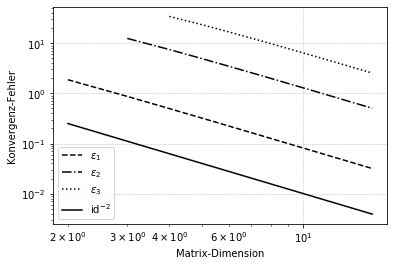
\includegraphics[width = 0.5 \textwidth]{Aufgabe_2/Konvergenz-Fehler_der_Eigenwerte_von_A_n}
  \caption{Konvergenz-Fehler der Eigenwerte von $A_n$}
  \label{Konvergenz-Fehler_EW}
\end{figure}

\textbf{Wenn wir mit dem plot von den Eigenvektoren fertig sind, dann kommt der auch noch hier her!}

\subsection{verallgemeinerte Eigenschwingungen}

Die Ausbreitungsgeschwindigkeit $c$ in \eqref{Wellengleichung} hängt vom Material der Saite ab. Bisher haben wir sie als konstant angenommen, d.h. die Saite bestand aus einem Material. Sei nun für $c_0, c_1 \in \R$

\begin{align} \label{Material-Funktion}
  c(x) :=
  \begin{cases}
    c_0, x \in (0, 1/2) \\
    c_1, x \in (1/2, 1)
  \end{cases}.
\end{align}

Zuerst leiten wir eine zur Helmholz-Gleichung \eqref{Helmholz-Gleichung} ähnliche Gleichung her und geben einen \eqref{Analytische_Lösung} entsprechenden Lösungsansatz an, wenn die Lösung $v$ auf $(0, 1)$ stetig differenzierbar sein soll.
Dabei betrachten wir eine angepasste Version der Wellengleichung \eqref{Wellengleichung}.

\begin{align*}
  \frac{\partial^2 u}{\partial x^2} (t, x) =
  \frac{1}{c^2(x)}
  \frac{\partial^2 u}{\partial t^2} (t, x), \qquad
  x \in (0, 1), \qquad
  t \in \R
\end{align*}

Wir verwenden jedoch den selben Ansatz, wie Vorher. Das war $u(x, t) = \mathfrak{R} (v(x) e^{-i \omega t})$, mit einer festen, aber unbekannten Kreisfrequenz $\omega > 0$ und einer Funktion $v$, welche nur noch vom Ort $x$ abhängt. \\

Einsetzen und analoges Nachrechnen, gibt mit der unbekannten Wellenzahl $\kappa(x) := \frac{\omega}{c(x)}$, die Randbedingungen \eqref{Randbedingungen} und

\begin{align} \label{Helmholz-Gleichung}
  -v^\primeprime(x) = \kappa^2(x) v(x), \qquad
  x \in (0, 1).
\end{align}

Um Probleme mit der Differenzierbarkeit von $\kappa$ zu vermeiden, führen wir die Abkürzungen $\kappa_0 := \frac{\omega}{c_0}$, $\kappa_1 := \frac{\omega}{c_1}$ ein. Wir definieren den Lösungsansatz durch Fallunterscheidung und mit (vorerst) beliebigen Konstanten $C_{01}, C_{02}, C_{11}, C_{12}$.

\begin{align*}
  v(x) :=
  \begin{cases}
    C_{01} \cos{(\kappa_0 x)} + C_{02} \sin{(\kappa_0 x)},
    & x \in (0, 1/2) \\
    C_{11} \cos{(\kappa_1 x)} + C_{12} \sin{(\kappa_1 x)},
    & x \in (1/2, 1)
  \end{cases}
\end{align*}

Durch Berücksichtigung der Randbedingungen \eqref{Randbedingungen}, erhält man (fast analog zu Vorher)

\begin{align*}
  C_{01} = 0, \qquad
  C_{11} \cos{\kappa_1} + C_{12} \sin{\kappa_1} = 0.
\end{align*}

Soll $v$ auf $1/2$ stetig fortgesetzt werden, so müssen dessen links- und rechts-seitiger Grenzwert übereinstimmen.

\begin{align*}
  C_{02} \sin(\kappa_0/2)
  = \lim_{x \to 1/2-} v(x)
  = \lim_{x \to 1/2+} v(x)
  = C_{11} \cos(\kappa_1/2) + C_{12} \sin(\kappa_1/2)
\end{align*}

Um stetige Differenzierbarkeit zu erhalten, muss auch die Ableitung

\begin{align*}
  v^\prime(x) =
  \begin{cases}
    C_{02} \kappa_0 \cos(\kappa_0 x),
    & x \in (0, 1/2) \\
    - C_{11} \kappa_1 \sin(\kappa_1 x) + C_{12} \kappa_1 \cos(\kappa_1 x),
    & x \in (1/2, 1)
  \end{cases}
\end{align*}

auf $1/2$ stetig fortgesetzt werden.

\begin{align*}
  \kappa_0 C_{02} \cos(\kappa_0/2)
  = \lim_{x \to 1/2-} v^\prime(x)
  = \lim_{x \to 1/2+} v^\prime(x)
  = - C_{11} \kappa_1 \sin(\kappa_1/2) + C_{12} \kappa_1 \cos(\kappa_1/2)
\end{align*}

Aus den Randbedingungen und stetigen Fortsetzungen, ergibt sich also das homogene lineare Gleichungssystem $R \vec C = 0$, mit

\begin{align*}
  R :=
  \begin{pmatrix}
    \sin(\kappa_0/2)          & -\cos(\kappa_1/2)         & -\sin(\kappa_1/2) \\
    \kappa_0 \cos(\kappa_0/2) & \kappa_1 \sin(\kappa_1/2) & - \kappa_1 \cos(\kappa_1/2) \\
    0                         & \cos{\kappa_1}            & \sin{\kappa_1}
  \end{pmatrix}
  \in \R^{3 \times 3}, \qquad
  \vec C :=
  \begin{pmatrix}
    C_{02} \\
    C_{11} \\
    C_{12}
  \end{pmatrix}
  \in \R^{3 \times 1}.
\end{align*}

Sei $R \in \GL[3]{\R}$ regulär, so ist deren Kern trivial, d.h. $\ker{R} = \Bbraces{0}$, und somit auch die Lösung $\vec C = 0$. Dieser Fall wäre jedoch wieder der trivialfall, darum betrachten wir den anderen Fall, also dass $\det{R} = 0$ gilt. Mit SymPy berechnet man

\begin{align*}
  \det{R} =
  \sin{\left(\frac{{\kappa}_{0}}{2} \right)} \cos{\left(\frac{{\kappa}_{1}}{2} \right)} {\kappa}_{1} + \sin{\left(\frac{{\kappa}_{1}}{2} \right)} \cos{\left(\frac{{\kappa}_{0}}{2} \right)} {\kappa}_{0}.
\end{align*}

Über $\kappa_0 = \frac{\omega}{c_0}$, $\kappa_1 = \frac{\omega}{c_1}$ lässt sich $\omega$, für gegebene $c_0$, $c_1$ als (nicht eindeutige) Nullstelle einer Funktion $f$ charakterisieren. Diese Überlegung, wird, in Form von folgender Funktion, implementiert.

\lstinputlisting
[language = Python]
{Aufgabe_2/python_code/get_zero_function.py}

Nun können wir $f$ für fixe $c_0, c_1$ plotten lassen. Dann bekommen wir ein besseres Verständnis dafür, welchen Startwert wir wählen sollen, um die Gleichung $f(\omega) = 0$, mit \verb|fsolve| aus \verb|scipy.optimize|, lösen zu lassen. \\

Für die folgenden Plots in Abbildung \ref{fig:zero_function}, wurden die arbiträren Werte $c_0 = 100$, $c_1 = 1$ gewählt. Die Funktion $f$ ist scheinbar gerade, d.h. symmetrisch bzgl. der $y$-Achse.

\begin{figure}[h!]
  \centering
  \subfloat[auf dem Intervall $(-16, 16)$]{
    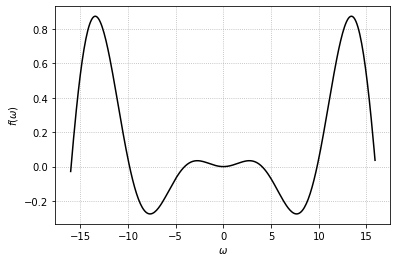
\includegraphics[width=65mm]{Aufgabe_2/zero_function_plot_c_0_100_c_1_1}
  }
  \subfloat[auf dem Intervall $(0, 100)$ und gezoomt]{
    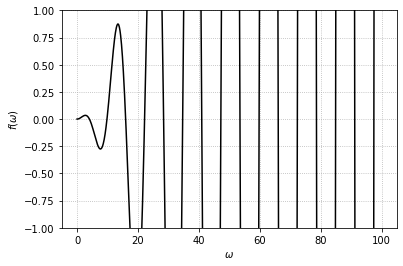
\includegraphics[width=65mm]{Aufgabe_2/zero_function_plot_c_0_100_c_1_1_zoomed}
  }
  \hspace{0mm}
  \caption{Plots von $f$ für $c_0 = 100$, $c_1 = 1$}
  \label{fig:zero_function}
\end{figure}

Dementsprechend, können passende Startwerte für iterative Verfahren gewählt werden. Die Ergebnisse vom, bereits erwähnten, \verb|fsolve| folgen. Warum die Quadrate dieser Ergebnisse eine Rolle spielen, wird später noch erwähnt.

\begin{multicols}{2}
\begin{verbatim}
solutions when guessing \omega = 0:
[0.]
squared:
[0.]

solutions when guessing \omega = 5:
[4.05742465]
squared:
[16.46269482]

solutions when guessing \omega = 10:
[9.82605835]
squared:
[96.55142264]

solutions when guessing \omega = 15:
[15.9568155]
squared:
[254.61996082]
\end{verbatim}
\end{multicols}

Wir wollen nun den Differenzenquotienten $D_h v(x_j)$, um ein verallgemeintertes Eigenwertproblem der Form $A \vec v = \lambda B \vec v$ mit Matrizen $A, B \in \R^{(n-1) \times (n-1)}$ herzuleiten. \\

Sei abermals $x_j := jh$, $j = 0, \ldots, n$ unsere Zerlegung des Intervalls $[0, 1]$ mit äquidistanter Schrittweite $h = 1/n$. Die Matrix $A_n$, für den Differenzenquotienten $D_h v(x_j)$ und der Vektor $\vec v := (v(x_1), \ldots, v(x_{n-1}))^T$, bleiben ebenfalls nach wie vor so, wie sie waren. \\

$B_n \lambda$ soll nun, analog zu Vorher, $-\kappa^2$ repräsentieren. Diesmal jedoch, ist $\kappa$ als Funktion zu verstehen. Also wird die Matrix $B_n$ deren Fallunterscheidungen übernehmen und $\lambda$ bleibt konstant. \\

\begin{align*}
  B_n :=
  \diag^{-2}
  (
    \underbrace{c_0, \ldots, c_0}_{\floor{\frac{n-1}{2}} \text{-mal}},
    \underbrace{c_1, \ldots, c_1}_{\ceil {\frac{n-1}{2}} \text{-mal}}
  ), \qquad
  \lambda := -\omega^2.
\end{align*}

Die Wahl von $B_n$ lässt sich wie folgt begründen: Für zwei Vektoren $a, b$, ist die Matrix-Vektor-Multiplikation $\cdot$, mit der Diagonalmatrix von $a$, äquivalent zur komponentenweisen Multiplikaiton $\odot$, d.h. $\diag(a) \cdot b = a \odot b$. Bei dem vorherigen Eigenwert-Problem wäre $B_n$ als die Einheits-Matrix $I_n$ zu betrachten, nachdem der Eigenwert $\lambda$ gleich ganz $-\kappa^2$ (konstant) übernehmen konnte. Da $-\kappa^2$ nun zwei Werte

\begin{align*}
  -\pbraces{\frac{\omega}{c_0}}^2, -\pbraces{\frac{\omega}{c_1}}^2
\end{align*}

annimmt, muss diese Eigenschaft von Diagonalmatrizen ausgenutzt werden, um die Unterscheidung zwischen $x_j < 1/2$ und $x_j \geq 1/2$ zu realisieren. \\

Wenn wir davon ausgehen, dass $c_0, c_1 \neq 0$, so ist $B_n$ wohldefiniert als Diagonalmatrix deren quadratische Kehrwerte. Damit lässt sich dieses verallgemeinerte Eigenwertproblem $A_n \vec v = \lambda B_n \vec v$, mit nahezu keinem Aufwand, in ein konkretes $B_n^{-1} A_n \vec v = \lambda \vec v$ umformulieren. \\

Dieses Eigenwertproblem wurde ebenfalls mit \verb|np.linalg.eig|, für beliebige $n \geq 2$, gelöst. Wir vergleichen die Eigenwerte und Eigenvektoren mit den oberen \glqq analytischen\grqq{} Ergebnissen mit $c_0 = 100$, $c_1 = 1$. Dass die Eigenwerte gegen $-\omega^2$ konvergieren, überrascht wenig. \\

\begin{verbatim}
n = 1000
-----
Eigenvalues:
-16.44054324040394
-96.3725475394107
-254.1214683324469
\end{verbatim}
